\chapter{Introduction}

Nepal is a country of extreme geographical and climatic diversity, compressed into a relatively small area. This unique combination, spanning from near sea level to the world's highest peaks, influences its climate, historical development, regional landscapes, and the lifestyles of its people. For a long, long time, Nepal's weather has decided where people settled down, what crops they grew, and even their festivals. The big summer rain, called the monsoon, is like the country's heartbeat. It brings most of the year's rain from June to September, helping farms grow food. The monsoon rains have grown more irregular and extreme over time causing floods and landslides, sometimes not enough leading to droughts. This is a big challenge, made worse by climate change affecting the whole world. The huge Himalayan mountains in the north also play a huge role. They block chilly winds from Central Asia in winter, and they catch all the monsoon rain, making some areas behind the mountains very dry

\section*{Terrain and its Influence on Climate}

Nepal's topography is arguably the most significant determinant of its climate. It's often divided into three distinct ecological belts running east to west:

\begin{enumerate}

\item \subsection*{Terai Region (Southern Lowlands)}

\textbf{Terrain:} This is a low-lying, flat, fertile plain, part of the Gangetic Plain, with elevations typically below 300 meters (around 1,000 feet). It includes some forested areas and gentle hill ranges (Siwalik Hills).\\
\textbf{Climate:} Experiences a tropical to subtropical monsoon climate. Summers are hot and humid, with temperatures often exceeding 37$^\circ$C (99$^\circ$F), and can even reach above 40$^\circ$C (104$^\circ$F) in some areas. Winters are mild, ranging from 7$^\circ$C to 23$^\circ$C (45$^\circ$F to 73$^\circ$F). The majority of rainfall occurs during the monsoon season (June to September), leading to lush vegetation but also prone to flooding.

\item \subsection*{Hilly Region (Mid-Hills)}

\textbf{Terrain:} Characterized by undulating hills, valleys (like Kathmandu and Pokhara Valleys), and ranges (Mahabharat Lekh), with altitudes generally between 800 to 4,000 meters (around 2,600 to 13,000 feet).\\
\textbf{Climate:} Features a warm temperate to cool temperate climate. Summers are generally pleasant (19$^\circ$C to 35$^\circ$C or 66$^\circ$F to 95$^\circ$F in valleys), while winters are cooler, with temperatures dropping to sub-zero at higher elevations. Kathmandu Valley has a moderate climate. This region also receives substantial monsoon rainfall, with some areas like Pokhara receiving very heavy rainfall due to the obstruction of monsoon clouds by the Annapurna range.

\item \subsection*{Himalayan Region (Northern Mountains)}

\textbf{Terrain:} Dominated by the Great Himalayan Range, including the world's highest peaks, with elevations ranging from 4,000 meters to over 8,848 meters (over 13,000 feet to 29,000 feet). This region includes high-altitude alpine valleys and vast snow-capped mountains.\\
\textbf{Climate:} Ranges from cool temperate to subarctic and arctic (or nival) climate. Summers are cool and short, while winters are severe, with temperatures consistently below freezing, often plunging to −25$^\circ$C (−13$^\circ$F) or lower at the highest altitudes. Snowfall is common, especially in winter. The Himalayas act as a massive barrier, blocking cold winds from Central Asia in winter and effectively trapping the monsoon winds from the south, leading to rain shadow areas (like Mustang and Manang) behind the main range which are arid or semi-arid.

\end{enumerate}
\section*{Lifestyle and Climate}

The diverse climate zones have directly shaped the lifestyles of the Nepali people:

\begin{enumerate}
  \item \textbf{Agriculture as a Core:} The majority of Nepal's population is engaged in subsistence agriculture, which is highly climate-dependent.
    \begin{itemize}
      \item In the Terai, tropical crops like rice, maize, and sugarcane are cultivated, benefiting from the warm, humid climate and monsoon rains.
      \item In the Hills, terraced farming is prevalent, allowing for the cultivation of a wider variety of crops suited to temperate conditions, including rice, maize, millet, wheat, and various vegetables.
      \item In the Himalayas, high-altitude communities rely on cold-tolerant crops like barley, buckwheat, and potatoes, along with pastoralism (yak herding) adapted to the harsh environment.
    \end{itemize}
  \item \textbf{Housing and Clothing:} Traditional architecture and clothing are adapted to local climatic conditions.
    \begin{itemize}
      \item Terai homes are often built with natural cooling in mind, using materials like mud, thatch, and bamboo. Lighter clothing is worn year-round.
      \item Hill homes are typically sturdier, often with stone or brick, providing insulation against cooler temperatures. Layered clothing is common.
      \item Himalayan houses are built to withstand extreme cold, using thick stone walls and often small windows. Warm, heavy woolens and animal hides are essential for survival.
    \end{itemize}
  \item \textbf{Cultural Practices and Festivals:} Many festivals and traditional practices are linked to the agricultural calendar and seasonal changes. For instance, festivals like Dashain and Tihar are celebrated after the monsoon harvest, reflecting gratitude for a successful crop.
  \item \textbf{Migration and Livelihoods:} Climate change impacts are increasingly affecting livelihoods. Unpredictable monsoons, droughts, and natural disasters are leading to reduced crop yields and food insecurity, especially in rural areas, prompting internal and external migration for alternative employment. Glacial melt threatens traditional livelihoods of Sherpa communities, forcing them to adapt or relocate.
  \item \textbf{Tourism:} The diverse climate zones also drive Nepal's tourism industry. Trekking and mountaineering are popular during the drier, clearer seasons (autumn and spring) when mountain views are optimal and temperatures are pleasant. Jungle safaris in the Terai are best during the dry winter months.
\end{enumerate}

\section*{Historical Perspective}

Historically, Nepal's climate has shaped human settlement patterns and interactions.

\begin{itemize}
  \item \textbf{Early Settlements and Trade Routes:} The fertile plains of the Terai and the milder mid-hills have long been the most welcoming places for people to live. These areas offered good soil and enough water to support farming, which helped early kingdoms and trading centers grow. The pleasant climate and reliable resources made it easier for communities to thrive and expand.

  \item \textbf{Mountain Barriers and Isolation:} The high Himalayan mountains in the north acted like a natural fortress, protecting the region but also keeping it isolated. This made it hard for outside influences to reach some mountain valleys, allowing unique cultures and traditions to develop in these remote areas. People there became largely self-reliant, shaped by the rugged environment around them.
  
  \item \textbf{Monsoon Dependence:}  For centuries, Nepal’s farming communities have depended heavily on the monsoon rains. The rhythm of planting, harvesting, and many cultural festivals has always followed the arrival of the monsoon. But when the rains are late, too light, or too heavy, it can cause serious problems like droughts, floods, or crop failures. These challenges have influenced migration patterns and the stability of communities over time.

  \item \textbf{Climate Change Impacts (Recent History):}  In recent decades, Nepal has been feeling the effects of global climate change more than most, even though it contributes very little to global emissions. Temperatures are rising, especially during the dry season, and rainfall is becoming less predictable. Winters are getting drier, while monsoon rains come in heavier bursts. These changes have led to more disasters like glacial lake floods, landslides, and severe droughts, which threaten the livelihoods of many, especially those who rely on farming and the natural environment.

\end{itemize}

\section*{Nepal’s Climatic Trends and Events}

Over the past few decades, Nepal’s climate has been changing noticeably. These changes are affecting everything from farming and water supply to wildlife and the everyday lives of people across the country.


\subsection*{Observed Climatic Trends in Nepal}

\begin{enumerate}

\item {Rising Temperatures}
\begin{itemize}
  \item According to the Department of Hydrology and Meteorology (DHM), Nepal’s average annual temperature has been increasing by approximately 0.06$^\circ$C per year since the 1970s. 
  \item The warming trend is more pronounced in the high Himalayan region compared to the lowlands. 
  \item Urban areas such as Kathmandu have experienced more frequent and prolonged heatwaves.
\end{itemize}

\item {Shifting Rainfall Patterns}
\begin{itemize}
  \item Monsoon rains, which account for over 80\% of annual precipitation, have become more erratic, with delayed onsets and sudden intense bursts. 
  \item There’s an observable increase in dry spells during the growing season and heavier rainfall over shorter periods, leading to increased risk of floods and landslides.
\end{itemize}

\item {Glacial Retreat} 
\begin{itemize}
  \item Glaciers in the Himalayas, including those feeding rivers like the Koshi and Gandaki, are retreating at alarming rates. 
  \item Studies show that more than 80\% of glaciers are shrinking, contributing to glacial lake outburst floods (GLOFs).
\end{itemize}

\item {Extreme Weather Events} 
\begin{itemize}
\item Nepal has seen a rise in extreme events like floods, landslides, droughts, and hailstorms over the past two decades. \item Changes in temperature and precipitation patterns have disrupted traditional farming calendars.
\end{itemize}
\end{enumerate}
\subsection*{Notable Climate-Related Events in Nepal}

\begin{longtable}{|p{4cm}|p{2cm}|p{8cm}|}
\hline
\textbf{Event} & \textbf{Year} & \textbf{Description} \\
\hline
\endfirsthead

\hline
\textbf{Event} & \textbf{Year} & \textbf{Description} \\
\hline
\endhead

Koshi Flood & 2008 & Breach in the Koshi embankment displaced over 70,000 people and caused massive destruction in the Terai. \\
\hline
Glacial Lake Outburst Flood (Dig Tsho) & 1985 & One of the earliest documented GLOFs in Nepal, causing loss of infrastructure and property in Khumbu. \\
\hline
Severe Drought in Mid-Western Nepal & 2009 & Affected food production and water supply, leading to a food crisis in many remote regions. \\
\hline
Melamchi Flash Flood & 2021 & Caused by intense rainfall and possible landslide dam bursts, severely damaging the Melamchi Water Project. \\
\hline
Rain-Induced Landslides & Recurring & Monsoon-triggered landslides are increasingly frequent in hill districts such as Sindhupalchok and Myagdi. \\
\hline
\end{longtable}
\captionsetup{justification=centering}
\captionof{table}{Major climate-related disasters in Nepal and their impact.}

\section*{Climate Science and Its Importance}

Climate science is the study of long-term patterns and changes in weather, temperature, and other atmospheric conditions on Earth. Unlike weather, which refers to short-term changes in the atmosphere, climate focuses on how these patterns evolve over decades, centuries, or even longer. Understanding climate science is crucial because it helps us understand the natural processes that shape our environment and how human activities, such as burning fossil fuels, affect these patterns.

Researchers in this field use sophisticated models and historical data to predict future climate changes. These predictions help in managing resources, preparing for extreme weather events, and making policy decisions to protect the planet and its inhabitants. Climate science is particularly important for several reasons:

\begin{itemize}
    \item \textbf{Human and Ecological Health:} Climate change has direct and indirect impacts on human health, including the spread of diseases, heatwaves, and the availability of clean water. Understanding climate patterns helps protect public health by predicting and mitigating these risks.
    \item \textbf{Natural Resource Management:} Climate science aids in managing natural resources like water, forests, and energy by predicting changes in the environment that might affect these resources. For instance, changes in precipitation patterns can influence water availability for agriculture and consumption.
    \item \textbf{Biodiversity Protection:} Climate science helps track how changing environmental conditions affect ecosystems and biodiversity. For example, many species are migrating or adapting to new climates due to rising temperatures, and understanding these changes is critical for protecting ecosystems.
    \item \textbf{Predicting and Preparing for Extreme Weather:} Climate scientists study the relationship between climate change and extreme weather events, such as hurricanes, floods, and wildfires. This helps in predicting these events and preparing communities, governments, and industries for their impacts.
\end{itemize}

In summary, climate science is essential for understanding the Earth’s natural systems and how human actions are influencing these systems. It provides the knowledge necessary for mitigating climate change, adapting to its effects, and making informed decisions for a sustainable future.

\section*{Data Analytics in Climate Science}

Data analytics plays a key role in climate science by transforming raw climate data into meaningful insights. Climate data is complex and often come in large volumes. Data analytics helps researchers and policy makers make sense of these data, uncover hidden trends, and make better decisions.

Here are a few ways data analytics is applied in climate science.

\begin{itemize}
    \item \textbf{Trend Analysis:} By analyzing historical climate data, scientists can identify long-term trends in temperature, precipitation, and other factors. For example, they might find that temperatures have been steadily rising in certain regions over the past 50 years.
    \item \textbf{Modeling and Predictions:} Climate models are created using statistical techniques to predict how climate will change in the future. These models use current and historical data to estimate future scenarios based on different levels of greenhouse gas emissions and other factors.
    \item \textbf{Visualization:} Data analytics tools such as graphs, maps, and charts help researchers and the public visualize complex climate data. Visualizations make it easier to understand trends, compare regions, and communicate findings.
    \item \textbf{Extreme Event Forecasting:} By analyzing patterns in weather data, data analytics can help predict extreme weather events such as hurricanes, droughts, and floods. This helps communities prepare and mitigate the effects of these events.
\end{itemize}

\section{Exploratory Data Analysis (EDA): A Simple Overview}

Exploratory Data Analysis (EDA) is the process of investigating and summarizing a dataset before jumping into more formal analysis or modeling. It helps us understand the data’s structure, detect patterns, and spot any issues like missing values or outliers. EDA uses statistical summaries and visual tools to gain insights, making it easier to build more accurate models later.

\subsection*{Types of Exploratory Data Analysis}

\subsubsection*{Univariate Analysis}  
This phase focuses on analyzing individual variables to understand their characteristics. Common techniques include:
\begin{itemize}
    \item Histograms: To visualize data distribution.
    \item Box Plots: For detecting outliers.
    \item Summary Statistics: Such as mean, median, mode, variance, and standard deviation.
\end{itemize}

\subsubsection*{Bivariate Analysis}  
Bivariate analysis examines relationships between two variables to identify correlations or dependencies. Techniques used include:
\begin{itemize}
    \item Scatter Plots: To visualize relationships between continuous variables.
    \item Correlation Coefficient: To quantify the strength of relationships.
    \item Cross-tabulation: For categorical variables.
\end{itemize}

\subsubsection*{Multivariate Analysis}  
This phase involves analyzing more than two variables simultaneously to explore complex interactions and relationships within the dataset. Common techniques include:
\begin{itemize}
    \item Pair Plots: To visualize pairwise relationships between multiple variables.
    \item Principal Component Analysis (PCA): To reduce the dimensionality of the data while retaining the most important features.
    \item Multiple Regression: To understand the relationship between one dependent variable and multiple independent variables.
\end{itemize}

\subsection*{Steps for Performing Exploratory Data Analysis (EDA)}

\begin{enumerate}
    \item \textbf{Understand the Problem and the Data:} First, we try to understand what the dataset is about and what questions we want to answer. For example, in climate data, we might want to know how temperature changes over months.
    
    \item \textbf{Import and Inspect the Data:} We load the data into tools like RStudio or Google Colab. Then, we inspect the structure — checking the number of rows, types of variables (numeric, categorical), and basic statistics like mean, median, and range.
    
    \item \textbf{Handle Missing Data:} Missing values are common in real-world data. We can handle them by techniques such as:
    \begin{itemize}
        \item Removing rows with missing values.
        \item Filling missing entries using mean, median, or mode (called imputation).
        \item Using more advanced methods like interpolation or prediction models.
    \end{itemize}
    
    \item \textbf{Explore Data Characteristics:} We perform basic statistical analysis to understand each variable. For example:
    \begin{itemize}
        \item Calculate mean, median, variance, and standard deviation.
        \item Create histograms and box plots to check data distribution and spot outliers.
    \end{itemize}
    
    \item \textbf{Perform Data Transformation:} Sometimes we need to adjust the data to make analysis easier. Common transformations include:
    \begin{itemize}
        \item Normalization: Scaling values between 0 and 1.
        \item Standardization: Adjusting data to have a mean of 0 and standard deviation of 1.
        \item Aggregation: Summarizing data, like taking the average monthly temperature from daily values.
    \end{itemize}
    
    \item \textbf{Visualize Data Relationships:} Visualization helps us see patterns that are hard to find in tables. We use:
    \begin{itemize}
        \item Scatter Plots: To explore relationships between two continuous variables.
        \item Bar Charts: To compare categories.
        \item Heatmaps: To visualize correlations among multiple variables.
        \item Line Charts: To show trends over time, especially in climate data.
    \end{itemize}
    
    \item \textbf{Handle Outliers:} Outliers are values that are much higher or lower than most data points. We can:
    \begin{itemize}
        \item Analyze if they are genuine observations.
        \item Correct or remove them if they are due to errors.
    \end{itemize}
    
    \item \textbf{Communicate Findings and Insights:} After analyzing the data, we summarize the key points through reports, graphs, and presentations. Clear communication makes the results understandable to everyone, even those who are not data experts.
\end{enumerate}

\begin{figure}[h]
\centering
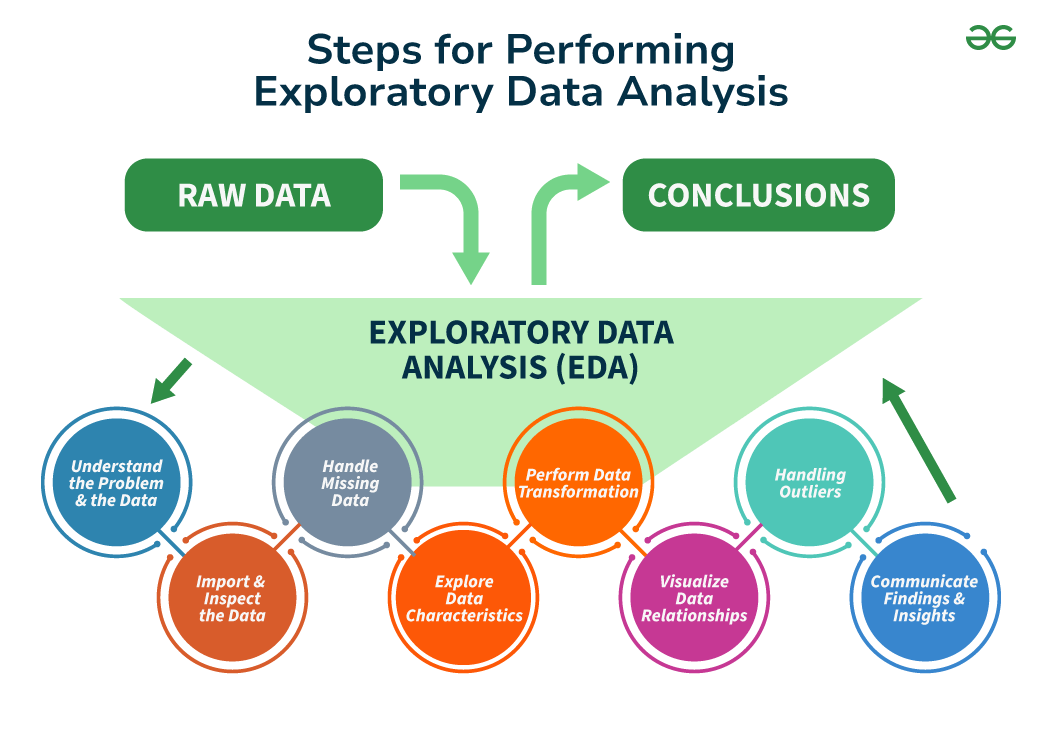
\includegraphics[width=0.6\textwidth]{figures/eda.png}
\caption{Steps of Performing EDA }
\end{figure}
For instance, if we want to explore climate data using Exploratory Data Analysis (EDA), we begin by loading the climate data, such as daily temperatures, into an analysis environment. The first step is to inspect the data for any missing values or errors. Next, we analyze the temperature distribution using histograms to determine whether the weather is mostly warm or cool. We also examine the relationship between temperature and other variables, like humidity, using scatter plots. In more complex cases, we explore how multiple factors, such as temperature, humidity, and wind speed, interact with each other. If we find missing data, we can either remove the affected entries or replace them with average values. Based on our analysis, we might identify trends, like rising temperatures over time, which could suggest climate change. Finally, we use visual tools such as scatter plots and heatmaps to clearly illustrate these relationships and communicate our findings. 
In this book, we will dive deeper into how to analyze climate data using these methods and explore additional techniques to uncover meaningful insights from real-world climate datasets.


\section{R Language for Data Analytics}

R is a widely-used programming language specifically designed for data analytics, statistical computing, and data visualization. It’s an excellent tool for exploring, analyzing, and interpreting complex datasets, making it highly suitable for various fields, including climate data analysis.

R excels in providing an extensive collection of packages and libraries that support tasks like data manipulation, statistical analysis, and generating visualizations. Some popular packages include \texttt{ggplot2} for data visualization, \texttt{dplyr} for data manipulation, and \texttt{tidyverse}, which bundles several powerful tools for data analysis. R is highly favored for its powerful statistical modeling capabilities and its ability to handle large datasets efficiently, which is especially useful when dealing with climate data or similar complex datasets.

The primary development platform for R is RStudio, an Integrated Development Environment (IDE) that provides an intuitive interface for coding, debugging, and visualizing data analysis results. RStudio makes it easier to write and execute R code by organizing the workspace into multiple panes for code writing, console output, and data visualizations. It offers features like code completion, a comprehensive help system, and a history of commands, which boosts productivity and efficiency in data analysis tasks.

Apart from RStudio, there are other platforms like JASP and Google Colab that can be used for data analytics. Google Colab is a cloud-based environment that enables R programming alongside Python. It allows easy access to resources without the need for local setup, making it a great choice for collaborative data science projects. Colab is especially useful for those who want to combine Python and R in a single workflow or need cloud-based resources for large-scale data analysis.

JASP (Jeffrey’s Amazing Statistics Program) is a free, open-source software platform designed for statistical analysis and data visualization. It integrates seamlessly with R, allowing for reproducible research, and is widely used in education and research due to its interactive features and visually appealing outputs. JASP is ideal for users who prefer a more interactive approach to data analysis without heavy reliance on coding, but still want powerful statistical analysis capabilities.

In this book, we will focus on leveraging R for data analytics, with a special emphasis on its applications for analyzing and visualizing climate data. We will explore how platforms like JASP and Google Colab can complement your analysis, making it easier to integrate multiple tools and enhance your analytical capabilities.

\section{Expanding Your R Toolkit with Packages}

Imagine R as a construction site where you’re building a house. The basic R installation gives you the essential tools—like a shovel and a measuring tape—to get started. However, as the project progresses, you need specialized machinery, such as a crane for lifting heavy materials, a cement mixer for mixing concrete, or a laser cutter for precise measurements. In R, packages are those specialized machines: they help you manage more complex tasks, streamline your workflow, and produce better, more accurate results. Without the right package, completing your project efficiently would be a lot harder.

\subsection{What are R Packages?}

An R package is a collection of reusable R functions, documentation that explains how to use them, and often sample data sets, all bundled together. Packages are created by the global R community and allow you to extend R’s capabilities far beyond the basics. Instead of writing complex code from scratch for every task, you can use a package designed specifically for that job.

\subsection{Finding and Using Packages}

Thousands of packages are available from online repositories, the main one being CRAN (The Comprehensive R Archive Network). You typically install a package once using the command:

\begin{verbatim}
install.packages("package name")
\end{verbatim}

Once installed, you need to load the package into your current R session to use its functions. Think of this like taking the specialized tool out of its box and putting it on your workbench. You do this using the command:

\begin{verbatim}
library(package name)
\end{verbatim}

Let’s explore some of the most useful and popular packages you’ll likely encounter. We’ll group them by the kind of tasks they help with.

\subsection{Core Data Science Tools: The tidyverse Ecosystem}

Many modern data analysis workflows in R rely on a collection of packages known as the \texttt{tidyverse}. These packages share a common design philosophy, making them work seamlessly together. Loading the main \texttt{tidyverse} package (\texttt{library(tidyverse)}) gives you access to several key packages at once.

\paragraph{dplyr: The Data Manipulator}

\textbf{What it Does:} Provides a set of core functions (called “verbs”) for the most common data manipulation tasks: subsetting, transforming, rearranging, and summarizing data stored in tables (data frames or tibbles).

\textbf{Why Use It?}
\begin{itemize}
    \item Intuitive Verbs: Functions have simple action-oriented names like \texttt{filter()} (keep rows based on conditions), \texttt{select()} (pick columns by name), \texttt{arrange()} (sort rows), \texttt{mutate()} (create or change columns) and \texttt{summarise()} (calculate summary statistics). This makes your code easy to write and understand.
    \item Readable Workflows: \texttt{dplyr} works beautifully with the pipe operator (\texttt{\%\textgreater\%} or the newer \texttt{|>}). This lets you chain operations together sequentially, making complex data transformations read like a set of instructions (e.g., \texttt{take data \%\textgreater\% then filter rows \%\textgreater\% then select columns}).
    \item Efficiency: Designed to be fast and efficient for most common data sizes you’ll work with directly in R.
    \item Consistency: As part of the tidyverse, it uses consistent rules and structures, making it easier to learn alongside other related packages.
\end{itemize}


\paragraph{ggplot2: The Grammar of Graphics}

\textbf{What it Does:} Implements the “Grammar of Graphics,” allowing you to build plots layer by layer. You start with your data, map variables to visual elements (like axes, colors, shapes), and then add geometric shapes (points, lines, bars, etc.).

\textbf{Why Use It?}
\begin{itemize}
    \item Power \& Flexibility: You can create a vast range of plot types, from simple scatter plots and bar charts to intricate multi-layered visualizations, all using the same core principles.
    \item High-Quality Output: Produces aesthetically pleasing, publication-quality graphics with sensible defaults.
    \item Customization: Offers deep control over every element of the plot.
    \item Logical Structure: Although it takes a little practice, the layered approach (\texttt{ggplot(...) + geom\_point() + labs(...)}) is a logical and consistent way to think about and build plots.
    \item Vibrant Community: Benefits from extensive online documentation, examples, and add-on packages for specialized plots.
\end{itemize}

\paragraph{tidyr: The Data Tidier}

\textbf{What it Does:} Helps you reshape your data into a “tidy” format. Tidy data has a consistent structure (each variable in a column, each observation in a row) that makes it easier to work with in R, especially within the tidyverse. Key functions help you pivot data between “wide” and “long” formats (\texttt{pivot\_wider()}, \texttt{pivot\_longer()}) or split/combine columns (\texttt{separate()}, \texttt{unite()}).

\textbf{Why Use It?}
\begin{itemize}
    \item Simplifies Cleaning: Addresses common messy data layouts, making data preparation much easier.
    \item Essential for tidyverse: Tidy data is the expected format for \texttt{dplyr} and \texttt{ggplot2}, so \texttt{tidyr} is often a crucial first step.
    \item Consistent Syntax: Follows the same design principles as other tidyverse packages.
\end{itemize}

\paragraph{readr: The Data Reader}

\textbf{What it Does:} Provides functions to read rectangular data from delimited text files like CSV (comma-separated values) and TSV (tab-separated values) into R.

\textbf{Why Use It?}
\begin{itemize}
    \item Speed: Often significantly faster than R’s built-in reading functions.
    \item User-Friendly: Gives helpful progress bars for large files and makes smarter guesses about column types.
    \item Modern Output: Reads data into tibbles, a modern type of R data frame used throughout the tidyverse.
    \item Sensible Defaults: Avoids common pitfalls like automatically converting text strings into factor variables.
\end{itemize}

\subsection{High-Performance Data Handling}

\paragraph{data.table: The Speed Demon}

\textbf{What it Does:} Provides an alternative way to work with data tables, optimized for speed and memory efficiency, especially with very large datasets.

\textbf{Why Use It?}
\begin{itemize}
    \item Speed: Can perform subsetting, grouping, joining, and updating operations much faster than dplyr or base R, particularly as data size grows.
    \item Memory Efficient: Uses clever techniques to modify data without making unnecessary copies, saving RAM.
    \item Concise Syntax: Uses a compact \texttt{DT[i, j, by]} syntax that can express complex operations in minimal code.
    \item Great for Big Data: The go-to package if you are pushing the limits of your computer’s memory or need maximum performance.
\end{itemize}

\subsection{Modeling and Machine Learning}

\paragraph{caret: The Modeling Workbench}

\textbf{What it Does:} Offers a unified interface for many tasks involved in machine learning: splitting data, pre-processing features, training various models using different algorithms, tuning model parameters, and evaluating performance.

\textbf{Why Use It?}
\begin{itemize}
    \item Unified Workflow: Provides a consistent set of functions (\texttt{train()}, \texttt{predict()}) to work with hundreds of different modeling techniques from various other R packages. This saves you from learning many different syntaxes.
    \item Streamlines Common Tasks: Simplifies processes like cross-validation, data preparation, and comparing model performance.
    \item Powerful and Feature-Rich: Offers extensive options for tuning and evaluating models.
\end{itemize}

\subsection{Specialized Utility Packages}

\paragraph{lubridate: The Date/Time Specialist}

\textbf{What it Does:} Simplifies working with date and time data, which can often be tricky. It provides easy functions for parsing dates/times from text, extracting components (like year, month, day, weekday), and doing calculations involving time.

\textbf{Why Use It?}
\begin{itemize}
    \item Intuitive Functions: Has memorable function names (e.g., \texttt{ymd()} to parse YearMonth-Day formats, \texttt{year()} to extract the year, \texttt{now()} to get the current time).
    \item Handles Complexity: Makes dealing with different formats, time zones, and date arithmetic much less error-prone than using base R functions alone.
    \item Essential for Time Series: Indispensable if your data involves timestamps or time-based analysis.
\end{itemize}

\paragraph{stringr: The Text Wrangler}

\textbf{What it Does:} Offers a consistent and simplified set of functions for common text manipulation tasks, such as detecting patterns (\texttt{str\_detect()}), replacing text (\texttt{str\_replace()}), splitting text into pieces (\texttt{str\_split()}), extracting parts of text (\texttt{str\_extract()}), and joining text together (\texttt{str\_c()}, \texttt{str\_glue()}).

\textbf{Why Use It?}
\begin{itemize}
    \item Consistency: Provides a cleaner, more predictable interface compared to base R’s string functions.
    \item Easier Regular Expressions: Simplifies the use of regular expressions (powerful pattern matching codes) for complex text tasks.
    \item tidyverse Friendly: Works well with the pipe operator and other tidyverse tools, making it great for cleaning text data within a larger workflow.
\end{itemize}

This list only scratches the surface! The beauty of R lies in this vast package ecosystem. As you encounter new tasks, chances are there’s a package out there designed to help. Don’t hesitate to search CRAN, read package documentation, and explore vignettes (package tutorials) to expand your R toolkit.